\documentclass{article}
\usepackage{listings}
\usepackage{graphicx}

\newcommand{\code}[1]{\lstinline{#1}}

\newcommand{\SolutionName}{InterfaceContracts}
\newcommand{\ProjectName}{InterfaceContracts}

\title{Interface Contracts Static Checking Example}
\date{}


\begin{document}
\maketitle
\begin{abstract}
This example shows how to use contracts on interfaces.
\end{abstract}

\newcommand\codefamily\sffamily
\lstset{language={[Sharp]C},mathescape=true,flexiblecolumns=true,morekeywords={Requires,Ensures,Invariant},basicstyle=\codefamily\small,literate={->}{{$\rightarrow$}}{2}{<<}{{$\langle$}}{2}{>>}{{$\rangle$}}{2}{!}{{\textbf{!}}}{2},frame=lines,moredelim=[is][\itshape]{@}{@},captionpos=b,numberstyle=\tiny,stepnumber=1,numbersep=2pt}

\section{Adding the Contract Library Reference}
If you are using Visual Studio 2008, or if you for 
some reason want to target a pre-v4 .NET runtime, then you need to:
\begin{itemize}
\item Change the target framework of the project.
\item Manually add a reference to Microsoft.Contracts.dll
\end{itemize}
Otherwise, you may skip this section and go directly the next section!

To add the reference, open the
\textsf{\SolutionName{}} solution and right-click on
\textsf{References} in the \textsf{\ProjectName{}} project and
select \textsf{Add Reference}. Find the \textsf{Microsoft.Contracts}
library in the \textsf{.NET} tab as shown below and click OK.
\begin{center}
  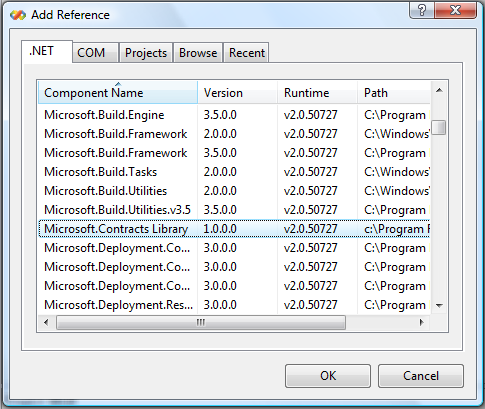
\includegraphics[width=.7\columnwidth]{../Common/addRef.png}
\end{center}



\section{Sample Walkthrough}
\label{sec:start}

After adding the proper reference, go to the Properties of project
\textsf{\ProjectName}, select the Code Contracts pane (at the bottom), and enable static
checking by clicking on the checkbox as shown in this screenshot:
\begin{center}
  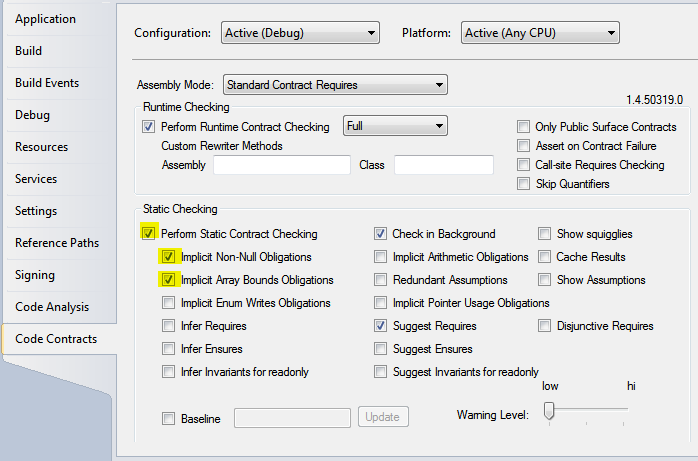
\includegraphics[width=.8\columnwidth]{ex1.png}
\end{center}

Then build the example. The static checker should warn about two
problems:
\begin{center}
  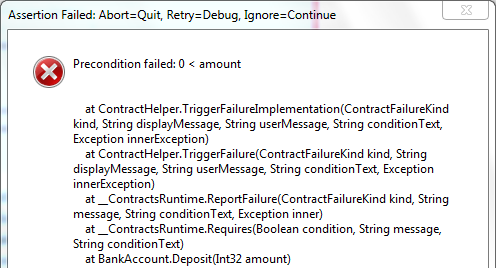
\includegraphics[width=1\columnwidth]{ex2.png}
\end{center}
The last problem in the list is in the call \code{f1.Foo(0)}. Given that
\code{FooImplementation1} implements interface \code{IFoo} and
\code{IFoo} has a contract written in the \code{IFooContract} class,
the \code{Foo} method of \code{FooImplementation1} automatically
inherits these contracts, namely:
\begin{lstlisting}
  Contract.Requires(x > 0);
  Contract.Ensures(Contract.Result<int>() > 0);
\end{lstlisting}
At the call site flagged by the checker, we are passing a value of 0,
which is clearly not positive.

Note how contracts are associated with an interface: take a look at
the interface declaration for \code{IFoo}. You see the attribute 
\begin{lstlisting}
  [ContractClass(typeof(IFooContract))]
\end{lstlisting}
This attribute informs the contract tools that the contract for
interface \code{IFoo} is to be found in the \code{IFooContract} dummy
class. Now look at the \code{IFooContract} class: it similarly has an
attribute stating what interface it annotates. This is for consistency
and documentation.
\begin{lstlisting}
  [ContractClassFor(typeof(IFoo))]
\end{lstlisting}
The return value
can be anything, or the methods can throw \code{NotImplementedException}.

Now take a look at the second error: it warns that the implementation
of \code{Foo} in class \code{FooImplementation2} is not conforming to
the \code{IFoo} contracts. Namely, the method may return 0, if the
argument is 1. Since the contract states that the return value should
be positive, the contract is not satisfied. In contrast,
\code{FooImplementation1} properly implements this contract, as it
returns the argument \code{x}, which is already known to be positive
given the precondition.

\end{document}
